\documentclass[border=4pt,12pt]{standalone}
% House style for redrawn exam diagrams (diagram-v4: 0.4pt lines, filled -latex arrows, fine dashes; stipple and hatching drawn as real dots/lines (no PDF/SVG patterns, so they render in every browser and at any scale); transparent background). Every figure \input's this.
\usepackage{amsmath,amssymb}
\usepackage{txfonts}
\usepackage{pdfrender,xcolor}
% \halo{text}: label on shading. The shading stops just around each letter's outline (a thin knock-out that follows the
% glyphs, like the papers' typesetting), never a box. Owner: "I don't want a box around the text".
\newcommand{\halo}[1]{\leavevmode\rlap{\pdfrender{TextRenderingMode=2,LineWidth=2.2pt,LineJoinStyle=1,StrokeColor=white,FillColor=white}#1}#1}
\usepackage{tikz,pgfplots}
\pgfplotsset{compat=1.18}
\usetikzlibrary{arrows.meta,calc,angles,quotes,patterns,patterns.meta,intersections,positioning,decorations.markings,shapes.geometric}
% Stipple and hatching are drawn as actual dots / lines clipped to the region (path picture), NOT as pattern fills:
% SVG <pattern> fills vanish or blur when browsers scale the image, so the owner could not see the shading.
% Each dot is a 0.72pt square (keeps SVGs small; reads as a dot at print size). Dots sit on one global staggered grid, so neighbouring regions line up.
\makeatletter
\newdimen\ex@x \newdimen\ex@y \newdimen\ex@xa \newdimen\ex@ya \newdimen\ex@xb \newdimen\ex@yb \newcount\ex@row
\def\exam@stipplecolor{black!75}\def\exam@dotr{0.42pt}\def\exam@dotgap{2.5}
\def\ex@rowdots{\ifdim\ex@x<\ex@xb \pgfpathrectangle{\pgfqpoint{\dimexpr\ex@x-0.36pt\relax}{\dimexpr\ex@y-0.36pt\relax}}{\pgfqpoint{0.72pt}{0.72pt}}\advance\ex@x by \exam@dotgap pt\relax\expandafter\ex@rowdots\fi}
\def\exam@stipple{%
  \pgftransformreset% dots are sized in real points even inside scaled pictures
  \pgfpointanchor{path picture bounding box}{south west}\ex@xa=\pgf@x \ex@ya=\pgf@y
  \pgfpointanchor{path picture bounding box}{north east}\ex@xb=\pgf@x \ex@yb=\pgf@y
  \pgfsetfillcolor{\exam@stipplecolor}\pgfmathsetmacro\ex@h{\exam@dotgap/2}%
  \pgfmathtruncatemacro\ex@r{floor(\ex@ya/\ex@h)-1}\ex@row=\ex@r\relax
  \ex@y=\ex@r\dimexpr\ex@h pt\relax
  \loop\ifdim\ex@y<\ex@yb
    \pgfmathtruncatemacro\ex@c{floor(\ex@xa/\exam@dotgap)-1}\ex@x=\ex@c\dimexpr\exam@dotgap pt\relax
    \ifodd\ex@row \advance\ex@x by \ex@h pt\fi
    \ex@rowdots
    \advance\ex@y by \ex@h pt \advance\ex@row by 1
    \ifnum\numexpr\ex@row-(\ex@row/4)*4\relax=0 \pgfusepath{fill}\fi% flush every 4 rows: bounded TeX memory, few clip copies in the SVG
  \repeat\pgfusepath{fill}}
\newdimen\ex@d
\def\exam@hatch#1{% #1 = 1 for /, -1 for \ ; lines 45 degrees, 3pt apart
  \pgftransformreset
  \pgfpointanchor{path picture bounding box}{south west}\ex@xa=\pgf@x \ex@ya=\pgf@y
  \pgfpointanchor{path picture bounding box}{north east}\ex@xb=\pgf@x \ex@yb=\pgf@y
  \ex@d=\dimexpr\ex@yb-\ex@ya\relax \ex@x=\dimexpr\ex@xa-\ex@d\relax
  \loop\ifdim\ex@x<\ex@xb
    \ifnum#1>0 \pgfpathmoveto{\pgfqpoint{\ex@x}{\ex@ya}}\pgfpathlineto{\pgfqpoint{\dimexpr\ex@x+\ex@d\relax}{\ex@yb}}%
    \else \pgfpathmoveto{\pgfqpoint{\ex@x}{\ex@yb}}\pgfpathlineto{\pgfqpoint{\dimexpr\ex@x+\ex@d\relax}{\ex@ya}}\fi
    \advance\ex@x by 4.24pt
  \repeat
  \pgfsetlinewidth{0.4pt}\pgfsetstrokecolor{black}\pgfusepath{stroke}}
\def\examstipple{\exam@stipple}\def\examhatch{\exam@hatch}\def\examsetstipplecolor#1{\def\exam@stipplecolor{#1}}\def\examsetdotgap#1{\def\exam@dotgap{#1}}
\makeatother
% (legacy pattern kept for old files)
% staggered stipple like the NESA papers' dotted shading
\pgfdeclarepatternformonly{exam stipple}{\pgfpointorigin}{\pgfqpoint{2.2pt}{2.2pt}}{\pgfqpoint{2.2pt}{2.2pt}}{%
  \pgfpathcircle{\pgfqpoint{0.55pt}{0.55pt}}{0.42pt}\pgfpathcircle{\pgfqpoint{1.65pt}{1.65pt}}{0.42pt}\pgfusepath{fill}}
\tikzset{
  every picture/.style={line width=0.6pt, >={Latex[length=2mm,width=1.3mm]}},
  curve/.style={line width=0.6pt},
  open arrow/.style={-{Latex[length=2mm,width=1.3mm]}},  % owner: filled -latex heads everywhere, no open chevrons
  aux/.style={dash pattern=on 2pt off 1.5pt, line width=0.6pt},
  shade/.code={\def\exA{#1}\def\exB{none}\ifx\exA\exB\else\pgfkeysalso{fill=black!18}\fi},
  shade/.default=on,
  shade dots/.style={fill=none, path picture={\examstipple}},
  stipple color/.code={\examsetstipplecolor{#1}},
  stipple gap/.code={\examsetdotgap{#1}},
  shade dense dots/.style={fill=none, stipple gap=1.6, path picture={\examstipple}},
  shade hatch/.style={fill=none, path picture={\examhatch{1}}},
  shade hatch reverse/.style={fill=none, path picture={\examhatch{-1}}},
  shade solid/.style={fill=black},
  pt/.style={circle, fill, inner sep=1.1pt},
  open pt/.style={circle, draw, fill=white, inner sep=1.1pt},
}
\pgfplotsset{
  exam axes/.style={axis lines=middle, axis line style={->}, xlabel={$x$}, ylabel={$y$},
    xlabel style={anchor=west}, ylabel style={anchor=south}, tick label style={font=\small},
    every axis plot/.append style={line width=0.6pt, black}, samples=200, clip=false,
    enlargelimits=false, axis on top},
}

\begin{document}
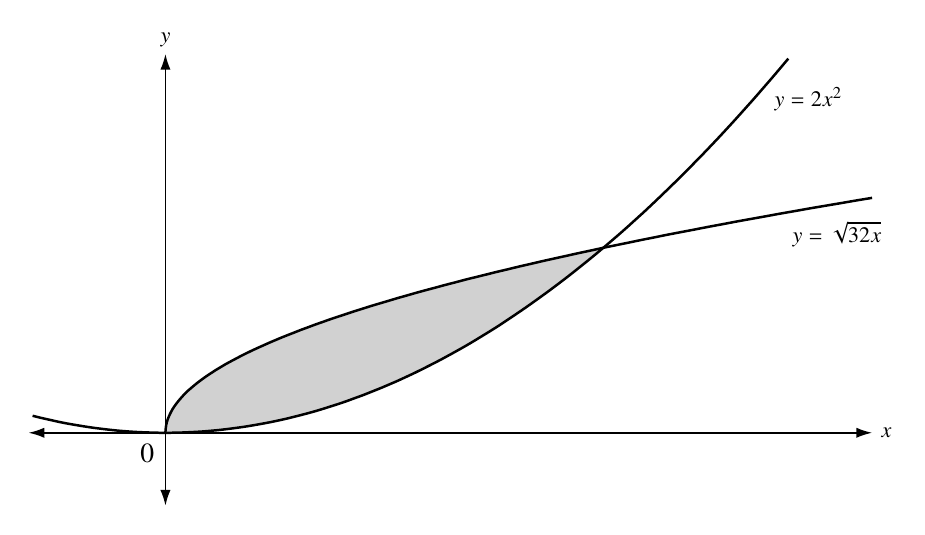
\begin{tikzpicture}[x=0.0127cm, y=-0.0127cm]
\fill[shade] plot[smooth] coordinates {(205.0,467.0) (205.1,463.9) (205.5,460.7) (206.1,457.6) (207.0,454.5) (208.1,451.3) (209.5,448.2) (211.2,445.1) (213.1,441.9) (215.2,438.8) (217.6,435.6) (220.2,432.5) (223.1,429.4) (226.3,426.2) (229.7,423.1) (233.3,420.0) (237.2,416.8) (241.4,413.7) (245.8,410.6) (250.4,407.4) (255.3,404.3) (260.5,401.2) (265.9,398.0) (271.6,394.9) (277.5,391.7) (283.6,388.6) (290.1,385.5) (296.7,382.3) (303.6,379.2) (310.8,376.1) (318.2,372.9) (325.9,369.8) (333.8,366.7) (342.0,363.5) (350.5,360.4) (359.1,357.3) (368.1,354.1) (377.3,351.0) (386.7,347.8) (396.4,344.7) (406.3,341.6) (416.5,338.4) (427.0,335.3) (437.7,332.2) (448.6,329.0) (459.8,325.9) (471.2,322.8) (482.9,319.6) (494.9,316.5) (507.1,313.4) (519.6,310.2) (532.3,307.1) (545.2,303.9) (558.4,300.8) (571.9,297.7) (585.6,294.5) (599.6,291.4) (613.8,288.3) (628.3,285.1) (643.0,282.0) (643.0,282.0) (635.6,288.2) (628.2,294.3) (620.7,300.3) (613.3,306.2) (605.9,312.0) (598.5,317.7) (591.0,323.3) (583.6,328.8) (576.2,334.1) (568.8,339.4) (561.3,344.6) (553.9,349.6) (546.5,354.5) (539.1,359.4) (531.6,364.1) (524.2,368.7) (516.8,373.3) (509.4,377.7) (501.9,382.0) (494.5,386.2) (487.1,390.3) (479.7,394.2) (472.3,398.1) (464.8,401.9) (457.4,405.6) (450.0,409.1) (442.6,412.6) (435.1,415.9) (427.7,419.2) (420.3,422.3) (412.9,425.3) (405.4,428.3) (398.0,431.1) (390.6,433.8) (383.2,436.4) (375.7,438.9) (368.3,441.3) (360.9,443.6) (353.5,445.7) (346.1,447.8) (338.6,449.8) (331.2,451.6) (323.8,453.4) (316.4,455.0) (308.9,456.6) (301.5,458.0) (294.1,459.3) (286.7,460.6) (279.2,461.7) (271.8,462.7) (264.4,463.6) (257.0,464.4) (249.5,465.1) (242.1,465.7) (234.7,466.1) (227.3,466.5) (219.8,466.8) (212.4,466.9) (205.0,467.0)} -- cycle;
\draw[<->] (68,467) -- (912,467);
\draw[<->] (205,540) -- (205,88);
\draw[line width=0.9pt] plot[smooth] coordinates {(72.1,450.0) (80.6,452.1) (89.1,454.0) (97.5,455.9) (106.0,457.6) (114.5,459.1) (123.0,460.5) (131.5,461.8) (140.0,462.9) (148.5,463.9) (157.0,464.8) (165.5,465.5) (174.0,466.1) (182.5,466.5) (191.0,466.8) (199.5,467.0) (208.0,467.0) (216.5,466.9) (225.0,466.6) (233.5,466.2) (242.0,465.7) (250.4,465.0) (258.9,464.2) (267.4,463.2) (275.9,462.1) (284.4,460.9) (292.9,459.5) (301.4,458.0) (309.9,456.4) (318.4,454.6) (326.9,452.7) (335.4,450.6) (343.9,448.4) (352.4,446.1) (360.9,443.6) (369.4,440.9) (377.9,438.2) (386.4,435.3) (394.8,432.2) (403.3,429.1) (411.8,425.7) (420.3,422.3) (428.8,418.7) (437.3,415.0) (445.8,411.1) (454.3,407.1) (462.8,402.9) (471.3,398.6) (479.8,394.2) (488.3,389.6) (496.8,384.9) (505.3,380.1) (513.8,375.1) (522.3,369.9) (530.8,364.7) (539.3,359.3) (547.7,353.7) (556.2,348.0) (564.7,342.2) (573.2,336.2) (581.7,330.1) (590.2,323.9) (598.7,317.5) (607.2,311.0) (615.7,304.3) (624.2,297.5) (632.7,290.6) (641.2,283.5) (649.7,276.3) (658.2,269.0) (666.7,261.5) (675.2,253.8) (683.7,246.1) (692.1,238.2) (700.6,230.1) (709.1,221.9) (717.6,213.6) (726.1,205.1) (734.6,196.5) (743.1,187.8) (751.6,178.9) (760.1,169.9) (768.6,160.7) (777.1,151.4) (785.6,141.9) (794.1,132.4) (802.6,122.6) (811.1,112.8) (819.6,102.8) (828.1,92.7)};
\draw[line width=0.9pt] plot[smooth] coordinates {(205.0,467.0) (205.1,464.4) (205.4,461.7) (205.8,459.1) (206.4,456.4) (207.2,453.8) (208.2,451.2) (209.4,448.5) (210.7,445.9) (212.2,443.2) (213.9,440.6) (215.8,438.0) (217.9,435.3) (220.1,432.7) (222.5,430.0) (225.1,427.4) (227.8,424.7) (230.8,422.1) (233.9,419.5) (237.2,416.8) (240.7,414.2) (244.4,411.5) (248.2,408.9) (252.2,406.3) (256.4,403.6) (260.8,401.0) (265.3,398.3) (270.1,395.7) (275.0,393.1) (280.1,390.4) (285.3,387.8) (290.8,385.1) (296.4,382.5) (302.2,379.9) (308.2,377.2) (314.3,374.6) (320.7,371.9) (327.2,369.3) (333.9,366.7) (340.7,364.0) (347.8,361.4) (355.0,358.7) (362.4,356.1) (370.0,353.4) (377.8,350.8) (385.7,348.2) (393.8,345.5) (402.1,342.9) (410.6,340.2) (419.3,337.6) (428.1,335.0) (437.1,332.3) (446.3,329.7) (455.7,327.0) (465.2,324.4) (475.0,321.8) (484.9,319.1) (495.0,316.5) (505.2,313.8) (515.7,311.2) (526.3,308.6) (537.1,305.9) (548.1,303.3) (559.2,300.6) (570.6,298.0) (582.1,295.3) (593.8,292.7) (605.6,290.1) (617.7,287.4) (629.9,284.8) (642.3,282.1) (654.9,279.5) (667.7,276.9) (680.6,274.2) (693.7,271.6) (707.0,268.9) (720.5,266.3) (734.2,263.7) (748.0,261.0) (762.0,258.4) (776.2,255.7) (790.6,253.1) (805.1,250.5) (819.8,247.8) (834.7,245.2) (849.8,242.5) (865.1,239.9) (880.5,237.3) (896.1,234.6) (911.9,232.0)};
\node[font=\footnotesize, anchor=west, inner sep=2pt] at (914,467) {$x$};
\node[font=\footnotesize, anchor=south, inner sep=2pt] at (205,88) {$y$};
\node[font=\normalsize, anchor=north east, inner sep=3pt] at (203,469) {$0$};
\node[font=\footnotesize, anchor=west, inner sep=2pt] at (808,133) {$y=2x^2$};
\node[font=\footnotesize, anchor=west, inner sep=2pt] at (826,268) {$y=\sqrt{32x}$};
\end{tikzpicture}
\end{document}
